
%----------------------------------------------------------------------------------------
%	PACKAGES AND OTHER DOCUMENT CONFIGURATIONS
%----------------------------------------------------------------------------------------

\documentclass[11pt, oneside]{Thesis} % The default font size and one-sided printing (no margin offsets)

\graphicspath{{Pictures/}} % Specifies the directory where pictures are stored

\usepackage{titlesec}
\usepackage[square, numbers, comma, sort&compress]{natbib} % Use the natbib reference package - read up on this to edit the reference style; if you want text (e.g. Smith et al., 2012) for the in-text references (instead of numbers), remove 'numbers' 
\hypersetup{urlcolor=blue, colorlinks=true} % Colors hyperlinks in blue - change to black if annoying
\title{\ttitle} % Defines the thesis title - don't touch this

\begin{document}

\frontmatter % Use roman page numbering style (i, ii, iii, iv...) for the pre-content pages

\setstretch{1.3} % Line spacing of 1.3

% Define the page headers using the FancyHdr package and set up for one-sided printing
\fancyhead{} % Clears all page headers and footers
\rhead{\thepage} % Sets the right side header to show the page number
\lhead{} % Clears the left side page header

\pagestyle{fancy} 

\newcommand{\HRule}{\rule{\linewidth}{0.5mm}} 
% PDF meta-data
\hypersetup{pdftitle={\ttitle}}
\hypersetup{pdfauthor=\authornames}




\titleformat
{\chapter} % command
[display] % shape
{\bfseries\Large\itshape} % format
{Kapitel \ \thechapter} % label
{0.5ex} % sep
{
    \vspace{1ex}
    \centering
} % before-code
[
\vspace{-0.5ex}%
]

\renewcommand{\bibname}{Referenser}


%----------------------------------------------------------------------------------------
%	TITLE PAGE
%----------------------------------------------------------------------------------------

\begin{titlepage}
\begin{center}

\textsc{\LARGE Uppsala universitet}\\[1.5cm] 
\textsc{\Large Operativsystem och Processorienterad Programmering}\\[0.5cm] 

\HRule \\[0.4cm] 
{\huge \bfseries \ttitle}\\[0.4cm] 
{\large 2015-06-07}\\[0.1cm] 
\HRule \\[1.5cm] 
 
\begin{minipage}{1.2\textwidth}
\begin{flushleft} \large
\emph{Projektrapport grupp 5: }\\

{\authornames} 
\end{flushleft}
\end{minipage}
 
\vfill
\end{center}

\end{titlepage}


%----------------------------------------------------------------------------------------
%	LIST OF CONTENTS/FIGURES/TABLES PAGES
%----------------------------------------------------------------------------------------

\pagestyle{fancy} % The page style headers have been "empty" all this time, now use the "fancy" headers as defined before to bring them back

\lhead{\emph{Innehåll}} % Set the left side page header to "Contents"
\tableofcontents % Write out the Table of Contents

%----------------------------------------------------------------------------------------
%	REPORT CONTENT - CHAPTERS
%----------------------------------------------------------------------------------------

\mainmatter % Begin numeric (1,2,3...) page numbering

\pagestyle{fancy} % Return the page headers back to the "fancy" style

% Include the chapters of the thesis as separate files from the Chapters folder
% Uncomment the lines as you write the chapters


\chapter{Inledning} 

\label{Inledning} 

\lhead{Kapitel 1. \emph{Inledning}} 

\emph{Swarm intelligence} är ett koncept som innebär att en grupp av organismer, helt utan en ledare i centrum och endast med begränsad individuell intelligens, i grupp kan lösa komplexa problem. Swarm intelligence har fått relevans inom datavetenskapen vid lösning av shortest path och travelling salesman-problemet\citep{Reference4}. I projektets inledande stadie så var tanken att simulera ett fält med två myrkolonier som konkurrerar med varandra. Det visade sig dock att det var en för invecklad och tidskrävande implementation med två myrstackar så fokus lades istället på att simulera endast en myrkoloni. I vår simulering kan myrorna hitta utplacerad mat och sedan ta tillbaka den till sitt bo. Myrorna hittar vägen till maten och tillbaka med hjälp utav att lämna och följa olika feromoner.

Vi har konstruerat ett system som är fullständigt concurrent och arbetar helt utan någon supervisor eller tidssynkronisering. Detta har åstadkommits genom att låta varje objekt i simuleringen vara en egen process där all kommunikation mellan processerna sker via \emph{message passing}.

Vi har i detta projekt utnyttjat \emph{actor-modellen} kraftigt och genom att använda en del oortodoxa metoder lyckats få koden lätthanterlig och även lyckats göra systemet fritt från deadlocks.

 



\chapter{Översikt över systemet}

\label{Systemet} 

\lhead{Kapitel 2. \emph{Översikt över systemet}}

Systemet ger användaren möjligheten att observera simuleringen av en virtuell myrkoloni i realtid.

Användaren startar simuleringen utan input-parametrar och systemet körs sedan automatiskt och kräver ingen interaktion från användaren. 
Vid första anblick kan myrkolonin uppfattas som simpel, men komplexiteten i simuleringen ligger i systemarkitekturen och de algoritmer myrorna använder sig av för att effektivisera hämtningen av mat. Systemarkitekturen kommer att presenteras mer detaljerat i en annan sektion av rapporten.

\section{Concurrency}

På grund av den höga nivån av autonomitet kombinerat med separationen mellan de olika processerna så är vi tvungna att använda så kallad \emph{event-driven programming}, vilket är när ett program styrs av externa händelser som inte går att kontrollera eller förutse. Ett exempel på det är vid programmering av användargränssnitt, då det inte går att förutspå när eller i vilken ordning användaren kommer att ge input till systemet. 

Vi använder actor-modellen då den ger oss bra möjligheter att på ett konceptuellt och effektivt sätt implementera event-driven programming. Vi kan i actor-modellen fokusera på en modul i taget utan att behöva ta hänsyn till hur de andra modulerna är implementerade. Det enda som behövs är ett meddelandeprotokoll som alla moduler följer.

Det är viktigt att påpeka att vi använder asynkron event-driven programming. Detta ger upphov till många problem då vi inte kan garantera att meddelandena kommer i rätt ordning. Problemen löses med hjälp av meddelandefiltrering, som innebär att en process väntar på ett specifikt meddelande innan den går vidare och buffrar de meddelanden som kvarstår. Varje process behöver då ha ett speciellt tillstånd när den accepterar alla nya förfrågningar.
Simuleringen skapar ofta deadlocks och vi har därför implementerat ett system för att åtgärda dessa. Metoden beskrivs mer detaljerat i kapitel \ref{ch:Implementation}.

\section{Systemdesign}

I figur \ref{fig:design} syns en schematisk överblick av systemarkitekturen. Alla moduler arbetar helt asynkront och all kommunikation mellan modulerna sker via medelanden.

\begin{figure}

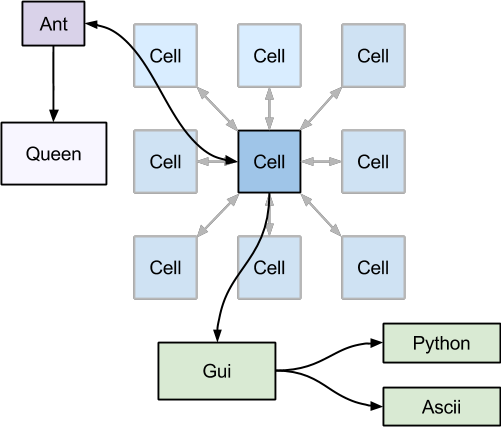
\includegraphics[scale=0.8]{Figures/systemdesign.png}
\caption{En schematisk överblick över systemarkitekturen}
\label{fig:design}
\end{figure}

\subsection{Ant}

Ant-modulen är den modul som implementerar myran. Ant-modulen innehåller de funktioner som krävs för att myran skall kunna fatta beslut över hur den ska agera baserat på hur dess omgivning ser ut. Myran skickar endast förfrågningar till den cell som den befinner sig på. Under normal drift så tar myran aldrig emot några förfrågningar från någon annan process, den tar endast emot svar från den cell som den befinner sig i.

Myran kommer på eget bevåg att skicka förfrågningar till den cellen den står på och autonomt att fatta beslut om vilken handling som är lämpligast, baserat på den informationen myran har tagit del av.

Ant-modulen är utrustad med funktionalitet så att myran kan analysera den information som ges av grannskapet till cellen den står i. Informationen gör det möjligt för myran att fatta ett beslut, baserat på vad myrans omgivning består av. Myror i det verkliga livet kommunicerar med varandra genom olika typer av feromoner, detta för att meddela var maten finns. Det är viktigt att myrorna kan inspektera sin omgivning så att den kan fatta ett beslut baserat på vad andra myror har upptäckt i omgivningen. Finns det feromoner som indikerar till myran att det finns föda i närheten kan myran ta ett beslut att röra sig i den riktningen och leta rätt på födan. Myrorna använder sig även av feromoner för att hitta hem till sitt näste. 


\subsection{Cell}

Cell-modulen representerar cellerna, varje cell är en ruta i det rutnät som utgör världen där myrorna lever. En cells primära uppgift är att ta emot och besvara förfrågningar från myran som står på cellen, samt de kringliggande cellerna. En cell kommer under normal drift aldrig att skicka en begäran till en annan cell, förutsatt att det är inte en begäran för att hantera en förfrågan som cellen har tagit emot. En cell kan endast skicka förfrågningar till de celler som är i dess direkta grannskap.

Cellen är det objekt som innehåller den relevanta informationen för systemet. En cell innehåller information om vad det är för typ av cell, om cellen exempelvis representerar ett myrbo: huruvida det finns mat på cellen, vad för intensitet de olika feromonerna har på cellen och om det står en myra på cellen.

Cellerna är de enda objekten som kommunicerar med GUI-modulen. När en cell får en förfrågan som förändrar cellens tillstånd skickar cellen ett meddelande till GUI-modulen där den talar om sin position och sitt nya tillstånd. 

\subsection{Message\_Buffer}

Message\_Buffer är den modul som hanterar kommunikationen av meddelanden mellan processerna. Modulen exporterar receiver-funktionen, funktionen är central för att använda den typ av event-driven programming som vi arbetar med. Receiver-funktionen används till våra metoder för att hantera deadlocks och filtrering av meddelandekön.

\subsection{GUI}

GUI-modulen är implementerad i Python och Erlang med hjälp av ErlPort. Modulen tar emot och behandlar meddelanden innehållandes cellernas tillstånd från cellerna. 
Informationen omvandlas till Pythons syntax via Erlport och skickas till en Python-instans som hanterar den grafiska representationen.

\subsection{Grid\_Init}

Modulen används för att bygga upp världen samt placera alla celler och länka ihop dessa. Grid\_Init modulen tilldelar även alla celler dess initiala attribut samt skapar, placerar och startar alla myrorna.

I denna modul initieras även en Queen-process, denna process binds alla myror till. Myrorna skickar statistik till Queen-processen, modulen är till för debugging och prestandamätning. 

\chapter{Implementation}

\label{ch:Implementation} 

\lhead{Kapitel 3. \emph{Implementation}}

\section{Programmeringsspråk}

Under den inledande fasen av projektet hade vi livliga diskussioner om vilket programmeringsspråk vi skulle använda. Vi bestämde att projektet skulle kretsa kring actor-modellen, det satte begränsningar på vilka språk vi kunde använda. Vi funderade först på att använda något nyutvecklat experimentellt språk och det stod mellan Nim och Rust. Efter mycket diskussion så skrotade vi denna idé då Nim\footnote{\url{http://nim-lang.org/}} är ett mycket nytt och instabilt språk, samtidigt som Rust\footnote{\url{http://www.rust-lang.org/}} är ett för strikt och invecklat språk. Användandet av Rust hade lett till att vi hade fått spendera mycket tid på lärandet av språket istället för att fokusera på de mer väsentliga delarna av projektet. 

Vi valde istället att använda Erlang för då det är ett väletablerat och stabilt språk byggt kring actor-modellen och message-passing. Utöver Erlang använde vi Python för den grafiska delen och ErlPort\footnote{\url{http://erlport.org/}} för kommunikationen mellan Erlang och Python. Implementationen av ErlPort har fungerat mycket bra och har gett oss ett smidigt interface mellan Erlang och Python.

\section{GUI}

GUI-modulen initieras med att skapa en lista motsvarande hela griden, den fylls med tomma atomer som Python-modulen inte ritar ut. GUI-modulen körs i en main loop som tar emot meddelanden från cell-modulerna, bearbetar dessa och fyller på den initierade listan. 

En algoritm används för att fördela listan på rätt X och Y koordinater, koordinaterna är angivna i meddelandet från cellen. Listan skickas via ErlPort till Python där den ritas upp grafiskt.

\subsection{Erlport}

Erlport är ett bibliotek som gör det möjligt för Erlang att kommunicera med andra programmeringsspråk. I dagsläget har Erlport stöd för Python och Ruby. 

För att Erlport ska kunna kommunicera med Python så skapar man först en instans, en Python instans är i princip en OS-process som representeras i Erlang av en Erlang process. Man kan skicka och ta emot medelanden mellan Erlang och Python på samma sätt som man skickar meddelanden mellan vanliga processer i Erlang.

\subsection{Pygame}

För den grafiska renderingen i projektet har vi använt oss av det community-utvecklade Pythonbiblioteket Pygame. Pygame är ett bibliotek av färdigutvecklade moduler till Python designade för att enkelt kunna skapa spel med en enkel grafisk implementation. Pygames design gör att det är enkelt att använda på alla plattformar som har stöd för Python.

\section{Ants and Cells}

Ant-modulen och Cell-modulen är väldigt lika varandra i sin implementation. Båda modulerna består utav en initialiseringsfunktion som används för att starta processer. Funktionen inväntar de meddelanden som är nödvändiga för att starta processerna. Detta kan till exempel vara ett meddelande om att myran har placerats korrekt och att cellerna har fått sitt grannskap definierat.

Cellerna och myrorna går efter ett meddelande till sin mainfunktion där de inväntar nya förfrågningar. Om det inte finns några obehandlade meddelanden kommer myrorna att agera spontant. När cellerna och myrorna får ett inkommande meddelande kommer de att anropa en funktion specifikt för den typen av meddelande. Dessa funktioner kan skicka och ta emot meddelanden själva med hjälp av meddelandefiltreringen. När en förfrågan eller annat meddelande har behandlats kommer processen återgå till sin mainfunktion. Om ett felaktigt eller otillåtet meddelande inkommer under någon del av exekveringen så kommer hela systemet att krascha.

Cellerna kommer vid varje inkommen förfrågan, beroende av cellens tillstånd, automatiskt genomföra en uppdatering av dess feromonnivåer. Detta sker som en funktion av den faktiska tiden(wall-time) som har gått sedan cellen senast uppdaterades.

Om en cell har attributet  \emph{block} så kan en myra inte gå dit och alla \verb+place_ant+ förfrågningar kommer att misslyckas.

\subsection{Myrans algoritm}

Myran beslut baseras på en väldigt enkel algoritm. Myran kan vara i två olika tillstånd \verb+searching_for_food+ och \verb+returning_with_food+. 

När myran letar efter mat så kommer den att undersöka cellen den står i, om det finns mat i cellen så kommer myran att försöka plocka upp maten. Om myran lyckas plocka upp mat kommer den att byta tillstånd till \verb+returning_with_food+, om myran misslyckas med att plocka upp mat så kommer den att fortsätta leta efter mat i andra celler.

När myran letar efter mat så kommer den att be cellen den står i att skicka tillbaka information om alla celler i dess grannskap. Myran kommer sedan att studera sitt grannskap och sortera cellerna efter hur mycket \verb+food_feremone+ varje cell innehåller och sedan genom \emph{rank-selection} att välja den riktingen den skall gå i. Rank-selection innebär att den med en förutbestämd sannolikhet $p$ kommer att gå till den cellen med det högsta antalet feromoner. Om den inte väljer den riktningen så kommer den att gå till den cellen med näst högst riktning med samma sannolikhet $p$.

Myran kommer efter varje genomförd förflyttning att släppa feromoner på den cellen där den tidigare var. Då myran letar efter mat kommer den att släppa \verb+base_feremone+ och då den går tillbaka med maten så kommer den att släppa \verb+food_feremone+.

Då myran går tillbaka med mat så kommer den att följa en snarlik algoritm men istället leta efter den högsta koncentrationen utav \verb+base_feremone+.

I figur \ref{fig:myralgo} finns en flow-chart om hur algoritmen ser ut.


\begin{figure}
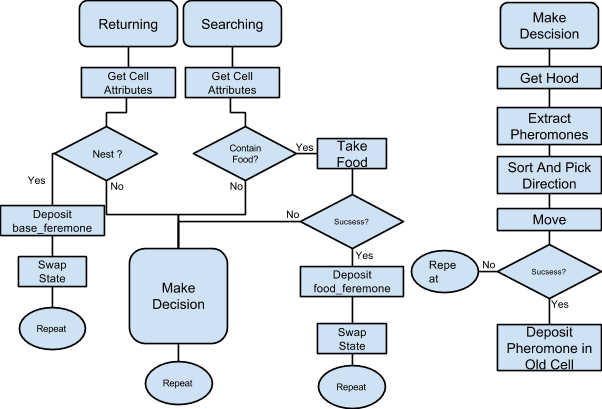
\includegraphics[scale=0.6]{Figures/myralgo.png}
\caption{Flowchart över myrans algoritm}
\label{fig:myralgo}
\end{figure}

\subsection{Grid\_Init}

Grid\_init är den modul som bygger upp världen. Det första som den modulen gör är att den startar alla cell-processer. Det krävs att GUI-modulen är startad, dess PID kommer att skickas med till alla celler. Den kommer sedan att skicka ut \verb+set_cell_attribute+ medelanden till alla dessa celler med cellernas attribut. Grid\_init kommer sedan att initiera en \emph{Queen}\footnote{Queen processen samlar in statistik från myrorna och används endast för debugging och testning.} process och starta alla myror och försöka placera ut dem på de celler där de skall starta. När alla myror har blivit utplacerade så kommer Grid\_init modulen att skicka \verb+start_ant+ medelanden till myrorna vilket kommer att starta simuleringen.

\section{Concurrency}

Då concurrencyn i vårat program uteslutande bygger på actor-modellen och message passing så har vi definierat tre klasser utav meddelanden.

\begin{itemize}

\item One-way meddelanden är på formen \verb+{Pid,{Type,Payload}}+ eller \verb+{Pid,Type}+
	One-way meddelanden är meddelanden som inte kommer att resultera i att något svar inkommer.

\item	Request (förfrågningar) meddelanden är på formen \verb+{Pid,Reference,Payload}+
	Alla Request-meddelanden resulterar i att processen blockerar och inväntar Reply-meddelanden.

\item	Reply-meddelanden är på formen \verb+{Pid,Refernce,Request_Reference,{Type,Reply_Payload}}+
	Reply-meddelanden är de meddelanden som skickas som svar på requests.

\end{itemize}


I alla meddelanden så är \verb+Pid+ att vara process id:t hos processen som skickar meddelandet \verb+Payload+ är vad meddelandet faktiskt innehåller  \verb+Reference+ är den referens som den skickade processen ger meddelandet \verb+Request_Reference+ är den referensen från ett request meddelande till vilket detta är ett svar.

Då systemet faller under \emph{ asynchronous event-driven programming} så kan vissa problem uppstå om vi inte är försiktiga med hur vi implementerar systemet. Det naiva tillvägagångssättet hade varit en så kallad \emph{Fifo, run to completion} metod. Detta innebär att man accepterar varje meddelande, hanterar det och låter det köra tills det att det är klart innan man hanterar nästa meddelande. Fifo-metoden leder dock till problem med att man måste hålla explicit koll på vilket tillstånd processen är i och ha en plan för hur man ska hantera alla kombinationer av meddelande-tillstånd. Detta skulle ha lett till extremt komplicerad och svårhanterlig kod.\citep{Reference5}

Lösningen på detta är att använda vad vi kallar för \emph{state-driven message handling}, vilket är att vi låter en process tillstånd diktera vilka meddelanden som den kommer att hantera. Det vi gör är att vi implementerar ett meddelandefilter som bara returnerar rätt meddelande (baserat på meddelandets unika tag/referens) och alla andra meddelanden som inkommer läggs på en buffer så att de senare kan hanteras.

Detta leder till att koden blir kortare och lättare att underhålla då vi på ett lätt sätt kan hantera hur systemet beter sig. Det finns dock ett krav på att alla processer måste ha ett eller flera tillstånd då de accepterar nya meddelanden. I detta tillstånd kommer meddelanden som ligger på buffern att hanteras först och när buffern är tom kommer de nya meddelandena att hanteras.


\subsection{Deadlocks}


Vår simulering är full av deadlocks och de uppstår ofta. Vi är därför tvungna att ha något system för att upptäcka och lösa alla deadlocks.

Vi kan för enklare deadlocks lösa detta effektivt och deterministiskt. Vi vet att om en process väntar på svar på en förfrågan så kommer den att blockera. Om en process väntar på ett svar från en annan process men får en förfrågan från den processen innan den har fått svar så vet vi att ett deadlock har uppstått. Processen som upptäcker att ett deadlock har uppstått kommer direkt att ge svar om misslyckande till den förfrågan som orsakade deadlocken. Det leder till att den andra processen kommer sluta blockera och förfrågan kan därefter hanteras. Detta förutsätter att det alltid är tillåtet för en förfrågan att misslyckas och att en process alltid kommer efter en finit tid kunna hantera nya förfrågningar efter det att en förfrågan har misslyckats.

Den här metoden kan bara endast lösa deadlocks som uppstår mellan två processer, men vi drabbas ständigt av mer komplicerade deadlocks i systemet.

Vi har konstruerat en metod för att lösa mer komplicerade distribuerade deadlocks som är väldigt simpel men mycket effektiv. Vår metod löser alla deadlocks helt automatiskt och kräver inte att några rollbacks \footnote{Att systemet återställs till ett tidigare tillstånd} måste genomföras eller analys av det globala tillståndet med en Wait-For-Graph.\citep{Reference6} Vår metod kräver inte heller att några \emph{probe} meddelanden skickas mellan processerana som i Chandy-Misra-Haas algoritmen.\citep{Reference7}

Dock så predikeras vår metod på en uppsättning krav på systemet.

\begin{itemize}
\item Alla förfrågningar kan misslyckas på ett väldefinierat sätt.

\item Alla processer kommer att invänta ett svar efter en förfrågan har skickats. 

\item Från det att ett svar på en förfrågan har inkommit kommer processen alltid att inom en finit tid drivas till ett tillstånd där den accepterar inkommande förfrågningar.
\end{itemize}

Dessa är en uppsättning preliminära predikat. Det kan finnas ytterligare begränsningar som vi har missat då de inte är applicerbara på vårt system. Även då dessa predikat kan förefalla vara hårda så innebär inte det att funktionaliteten drabbas signifikant. De tillåter att en process som väntar på ett svar fortfarande kan hantera vissa meddelanden och skicka nya förfrågningar till processer. De tillåter även att man implementerar en prioritering utav olika typer av förfrågningar eller olika typer av processer.

När en process väntar på svar från en annan process så kommer den att efter en viss förutbestämd tid (timeout), skicka automatiska fail-svar till alla inkomna förfrågningar som ligger på dess meddelande-buffer. Detta kommer att repeteras tills att ett svar har inkommit. Ni kan se en schematisk beskrivning av algoritmen i figur \ref{fig:receiver}.

\begin{figure}
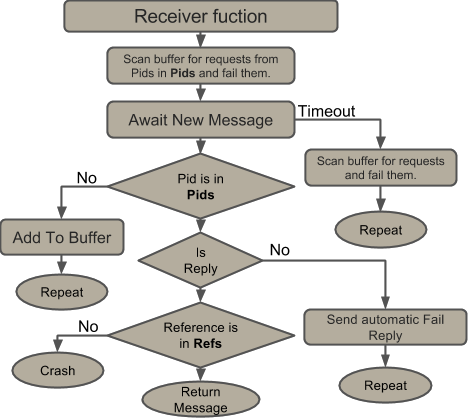
\includegraphics[scale=0.8]{Figures/receiver.png}
\caption{En schematisk överblick över hur meddelandefiltreringen och deadlock-hanteringen fungerar. \textbf{Refs} är en lista med de referenser från de förfrågningar meddelanden som har skickats.  \textbf{Pids} är en lista med de Pids som förfrågningarna har skickats till.}
\label{fig:receiver}
\end{figure}

Vår metod har dock den nackdelen att den ofta kommer att upptäcka \emph{falska deadlocks}, det vill säga att den kommer att tro att det finns ett deadlock när det inte gör det och i onödan avvisa vissa förfrågningar. Detta leder till att \textbf{Timeout} parametern måste finjusteras. En timeout som är för lång kommer innebära att deadlocks kommer att ligga kvar för länge innan de upptäcks och delar utav simuleringen kommer att  \emph{lagga}. En för kort timeout kommer att leda till att väldigt många förfrågningar kommer att avisas i onödan vilket också kan påverka systemets prestanda.
























 
\chapter{Slutsatser}

\label{Slutsats} 

\lhead{Kapitel 4. \emph{Slutsatser}}

Vi har lyckats göra en representation av en myrkoloni som samlar mat och kommunicerar med varandra med hjälp av feromoner. Myrorna kan även undvika olika hinder och objekt.  Även om vi inte riktigt lyckades implementera allt vi hade i åtanke när projektet började så är vi nöjda med slutresultatet. Det är svårt att få en verklig uppfattning av problemen och utmaningarna med ett arbete innan man satt igång med grunden på vilken andra implementationer ska vila. 
Vi bestämde oss för att se till att göra en grundläggande representation av en myrkoloni och se till att denna har god concurrency och en felfri körning, detta har vi uppnåt och även utvecklat en grafisk representation  Det är detta som vi nämnde tidigare, som är vår grund. På denna grund kan man enkelt bygga ut och genom detta implementera flera funktioner, som till exempel flera olika typer av mat, fientliga insekter och en konkurrerande myrkoloni.
Även om vår första tanke var att använda det nya och lite mer spännande språket Nim, så är vi nöjda med att vi valde att använda det mer utvecklade och etablerade språket Erlang. De verktyg som Erlang har tillgängliga har varit hjälpsamma och det är ett intressant språk att skriva i och actor-modellen är lätthanterlig för den här typen av concurrency.  

Sammanfattningsvis så har systemet levt upp till de förväntningar som gruppen hade haft i projektets tidiga stadie. 
 


%----------------------------------------------------------------------------------------
%	REPORT CONTENT - APPENDICES
%----------------------------------------------------------------------------------------

\titleformat
{\chapter} % command
[display] % shape
{\bfseries\Large\itshape} % format
{Appendix \ \thechapter} % label
{0.5ex} % sep
{
    \vspace{1ex}
    \centering
} % before-code
[
\vspace{-0.5ex}%
]

\addtocontents{toc}{\vspace{2em}} % Add a gap in the Contents, for aesthetics

\appendix % Cue to tell LaTeX that the following 'chapters' are Appendices

% Include the appendices of the thesis as separate files from the Appendices folder
% Uncomment the lines as you write the Appendices

\chapter{Utveckling}

\label{Utveckling} 

\lhead{Appendix A. \emph{Utveckling}}

Vi har använt Erlang(OTP 17.5) för den bakomliggande system-arkitekturen som hanterar myrornas AI samt cellstrukturen för simuleringen. Den grafiska represenattionen av systemet är skriven i Python(v 3.4) med hjälp av Pygame(1.9.1)\footnote{\url{http://www.pygame.org/news.html}}. Kommunikationen mellan Erlang och Python har skett med ErlPort(v 1.0.0 alpha)\footnote{\url{http://erlport.org/}}. Vi har använt EUnit\footnote{\url{http://www.erlang.org/doc/man/eunit.html}} för automatisering utav tester och EDoc för att generera dokumentation. Systemet byggs med hjälp av Make.


Vi har använt Github för hantering utav källkoden. Repot är just nu privat och är därför inte allmänt tillgängligt.



\chapter{Katalogstruktur}

\label{Katalogstruktur} 

\lhead{Appendix B. \emph{Katalogstruktur}}


Projektet är indelat i 4 huvudsakliga kataloger.

\begin{itemize}

\item doc     I denna mapp sparas projektets dokumentation. I \verb+html/+ kommer dokumentationen generad med EDoc att ligga. I \verb+pdf/+ katalogen ligger dokumentation i pdf format. I \verb+src/+ ligger källkodsfilerna till rapporten och projektförslaget.

\item ebin      I denna mapp finns .beam filerna. \textbf{OBS!} I denna mapp ligger även \verb+xd.py+ som är pythonfilen för GUI:t. Den måste ligga i denna mapp för att erlang skall hitta den.

\item meta    Denna mapp innehåller mötesprotokoll, gruppkontrakt och dagböcker.

\item src     Denna mapp innehåller källkoden till alla erlang-moduler. Src katalogen är indelad i underkataloger där varje modul har sin egen katalog med sina källkodsfiler.

\end{itemize}



\chapter{Installation}

\label{Installation} 

\lhead{Appendix C. \emph{Installation}}

Programmet byggs genom att köra \verb+make all+.
För att starta ascii Gui:t så skriver man \verb+make run_ascii+.
För att köra Python Gui:t så måste man gå till  \verb+ebin/+ katalogen och i erlang-tolken köra \verb+gui:initGui().+. Detta då erlang inte laddar python modulerna på ett korrekt sätt ananrs.

För att kunna starta Python gui:t krävs även att man har installerat Erlport 1.0.0, Python 3.x och Pygame 1.9.

\chapter{Reflektioner}

\label{Reflektioner} 

\lhead{Appendix D. \emph{Reflektioner}}

De flesta i gruppen hade inte någon större erfarenhet av Erlang förutom dem problemen vi fick lösa i problem set 3 i den här kursen. Sedan har vi ju även använt Python för det grafiska gränssnittet, Python var de flesta väldigt obekanta med så även det språket har samtliga i gruppen fått en bättre förståelse för. 

Utöver de språkliga kunskaper vi fått, är något vi kommer ta med oss från det här projektet hur man bäst kan utnyttja dynamiken i gruppen för att få arbete gjort så effektivt som möjligt. Tilldela de som är säkra på hur något moment skall göras med någon som är mindre erfaren och på så sätt förbereda denna för nästa liknande moment i projektet. Detta hade vi kunnat implementerat mer, men för att få detta tillväga gångssätt att fungera så måste alla i gruppen vara öppna och förmedla detta till samtliga i gruppen för att gruppen sedan ska bestämma en fungerande uppdelning av gruppen inför momentet. 

Vi har även varit noga med att utnyttja Scrum-metoden, med många korta möten där alla delat vad de haft för problem under veckan och vad de håller på med i dagsläget. Detta har varit väldigt hjälpsamt vid utvecklingen av systemet.

Ett streck i räkningen har varit att hålla samtliga i gruppen uppdaterad med vad för implementation som stundar. Detta har dock inte lett till några förseningar då det varit enkelt att få tag på alla i gruppen om någon haft frågor angående projektet. 
Sedan har gruppen varit svår att samla flera gånger per vecka på grund av krockande scheman, i projektets inledande stadie var vår tanke att vi skulle ses varje vardag under lunchen för att hålla alla uppdateringar och ha en sorts workshop där det är öppet för frågor inom gruppen.

Hade vi kunnat göra om projektet instämmer alla att vi borde ha nyttjat trello mer. Detta skulle ha underlättat synkronisationen av arbetet. Även om vi använde github flitigt så hade vi kunnat använda det till att se till att vi code-reviewade mer frekvent då det fanns många stavfel i koden kvar långt in i projektets gång. 
Som vi nämnde tidigare hade fler dagliga möten varit väldigt praktiskt då det hade gett mer rutin i arbetet. De flesta hade kunnat arbeta samtidigt vilket också hade underlättat kommunikationen

Slutligen hade vi kunnat ha använda Slack mer, då det är väldigt enkelt att citera och dela kod sinsemellan utan att behöva commita eller adda något till git repositoriet. Det kan också användas som en chatclient och det skulle leda till mindre distraktioner än att använda facebook för detta. 

\addtocontents{toc}{\vspace{2em}} % Add a gap in the Contents, for aesthetics

\backmatter

%----------------------------------------------------------------------------------------
%	BIBLIOGRAPHY
%----------------------------------------------------------------------------------------

\label{Bibliography}

\lhead{\emph{Referenser}} % Change the page header to say "Bibliography"

\bibliographystyle{unsrtnat} % Use the "unsrtnat" BibTeX style for formatting the Bibliography

\bibliography{Bibliography} % The references (bibliography) information are stored in the file named "Bibliography.bib"

\end{document}